\section{An initial overview of the course}
\title[Initial overview]{Initial Overview}

%%%%%%%%%%%%%%%%%%%%%%%%%%%%%%%%%%%%%%%%%%%%%%%%%%%%%%%%%%%%%
%% Overview of the course %%
%%%%%%%%%%%%%%%%%%%%%%%%%%%%%%%%%%%%%%%%%%%%%%%%%%%%%%%%%%%%%
\begin{frame}
	\frametitle{Course Overview}
The course contains the following 6 modules:
		\begin{itemize}
		  \item Module I:  Introduction to Automation Technologies.
		  \item Module II: Sensor Technologies.
		  \item Module III: Signal Processing and Conditioning.
		  \item Module IV: Processors Technologies in Automation Systems.
		  \item Module V: Industrial Communication in Automation Systems.
		\end{itemize}
\textbf{Pattern of class}: \\ Day: Tuesday, every week \\ 
Time: 8 am to 10 am (theory) and 10 am to 12 am (tutorial) (ideally but it can change) \\
Holidays: 23 Dec 2025, 30 Dec 2025, and 6 Jan 2026. %As required classes will be rescheduled. 
\end{frame}

%%%%%%%%%%%%%%%%%%%%%%%%%%%%%%%%%%%%%%%%%%%%%%%%%%%%%%%%%%%%%
%% Teaching Support Team %%
%%%%%%%%%%%%%%%%%%%%%%%%%%%%%%%%%%%%%%%%%%%%%%%%%%%%%%%%%%%%%
\begin{frame}
	\frametitle{The teaching team}
	\vspace{-0.5cm}
	\begin{columns}[t]
\centering
		\column[T]{0.33\textwidth}
		\begin{figure}
			\centering
				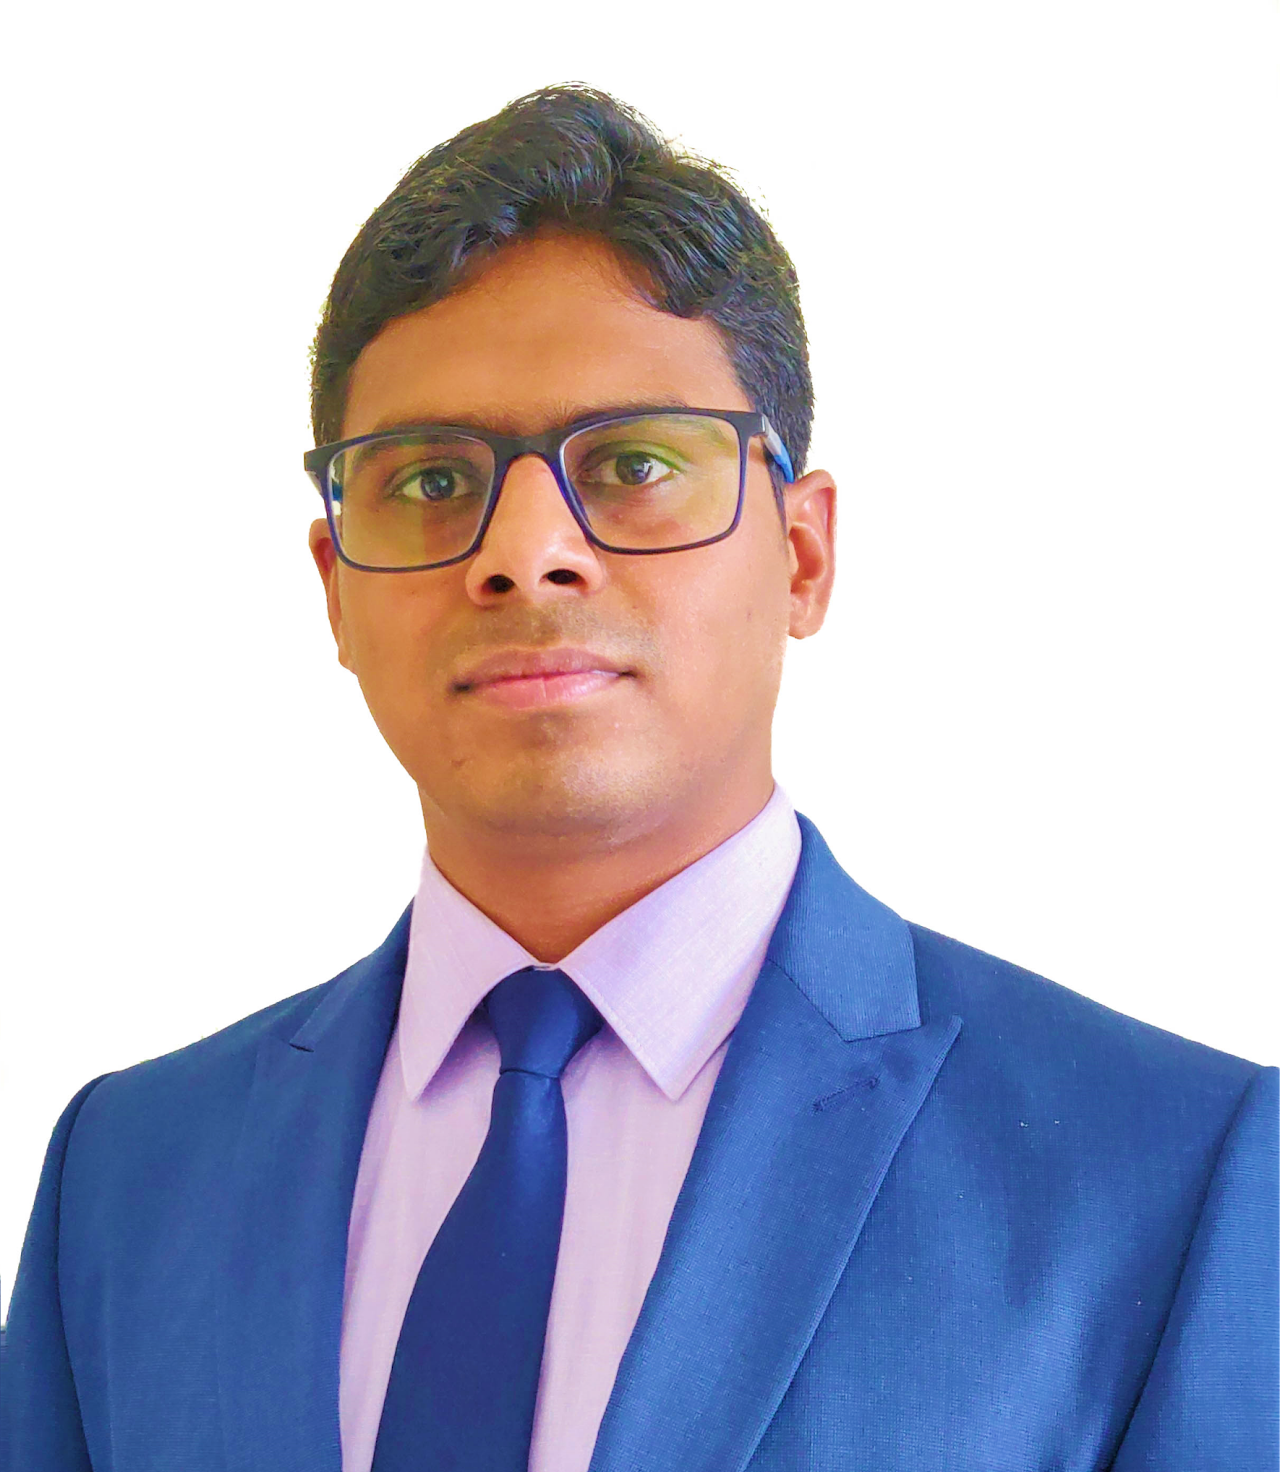
\includegraphics[height=2.5cm]{fig/lec01/Bikash.png}
				\caption*{Bikash Sah}
		\end{figure}
	
		\column[T]{0.33\textwidth}
		\begin{figure}
			\centering
				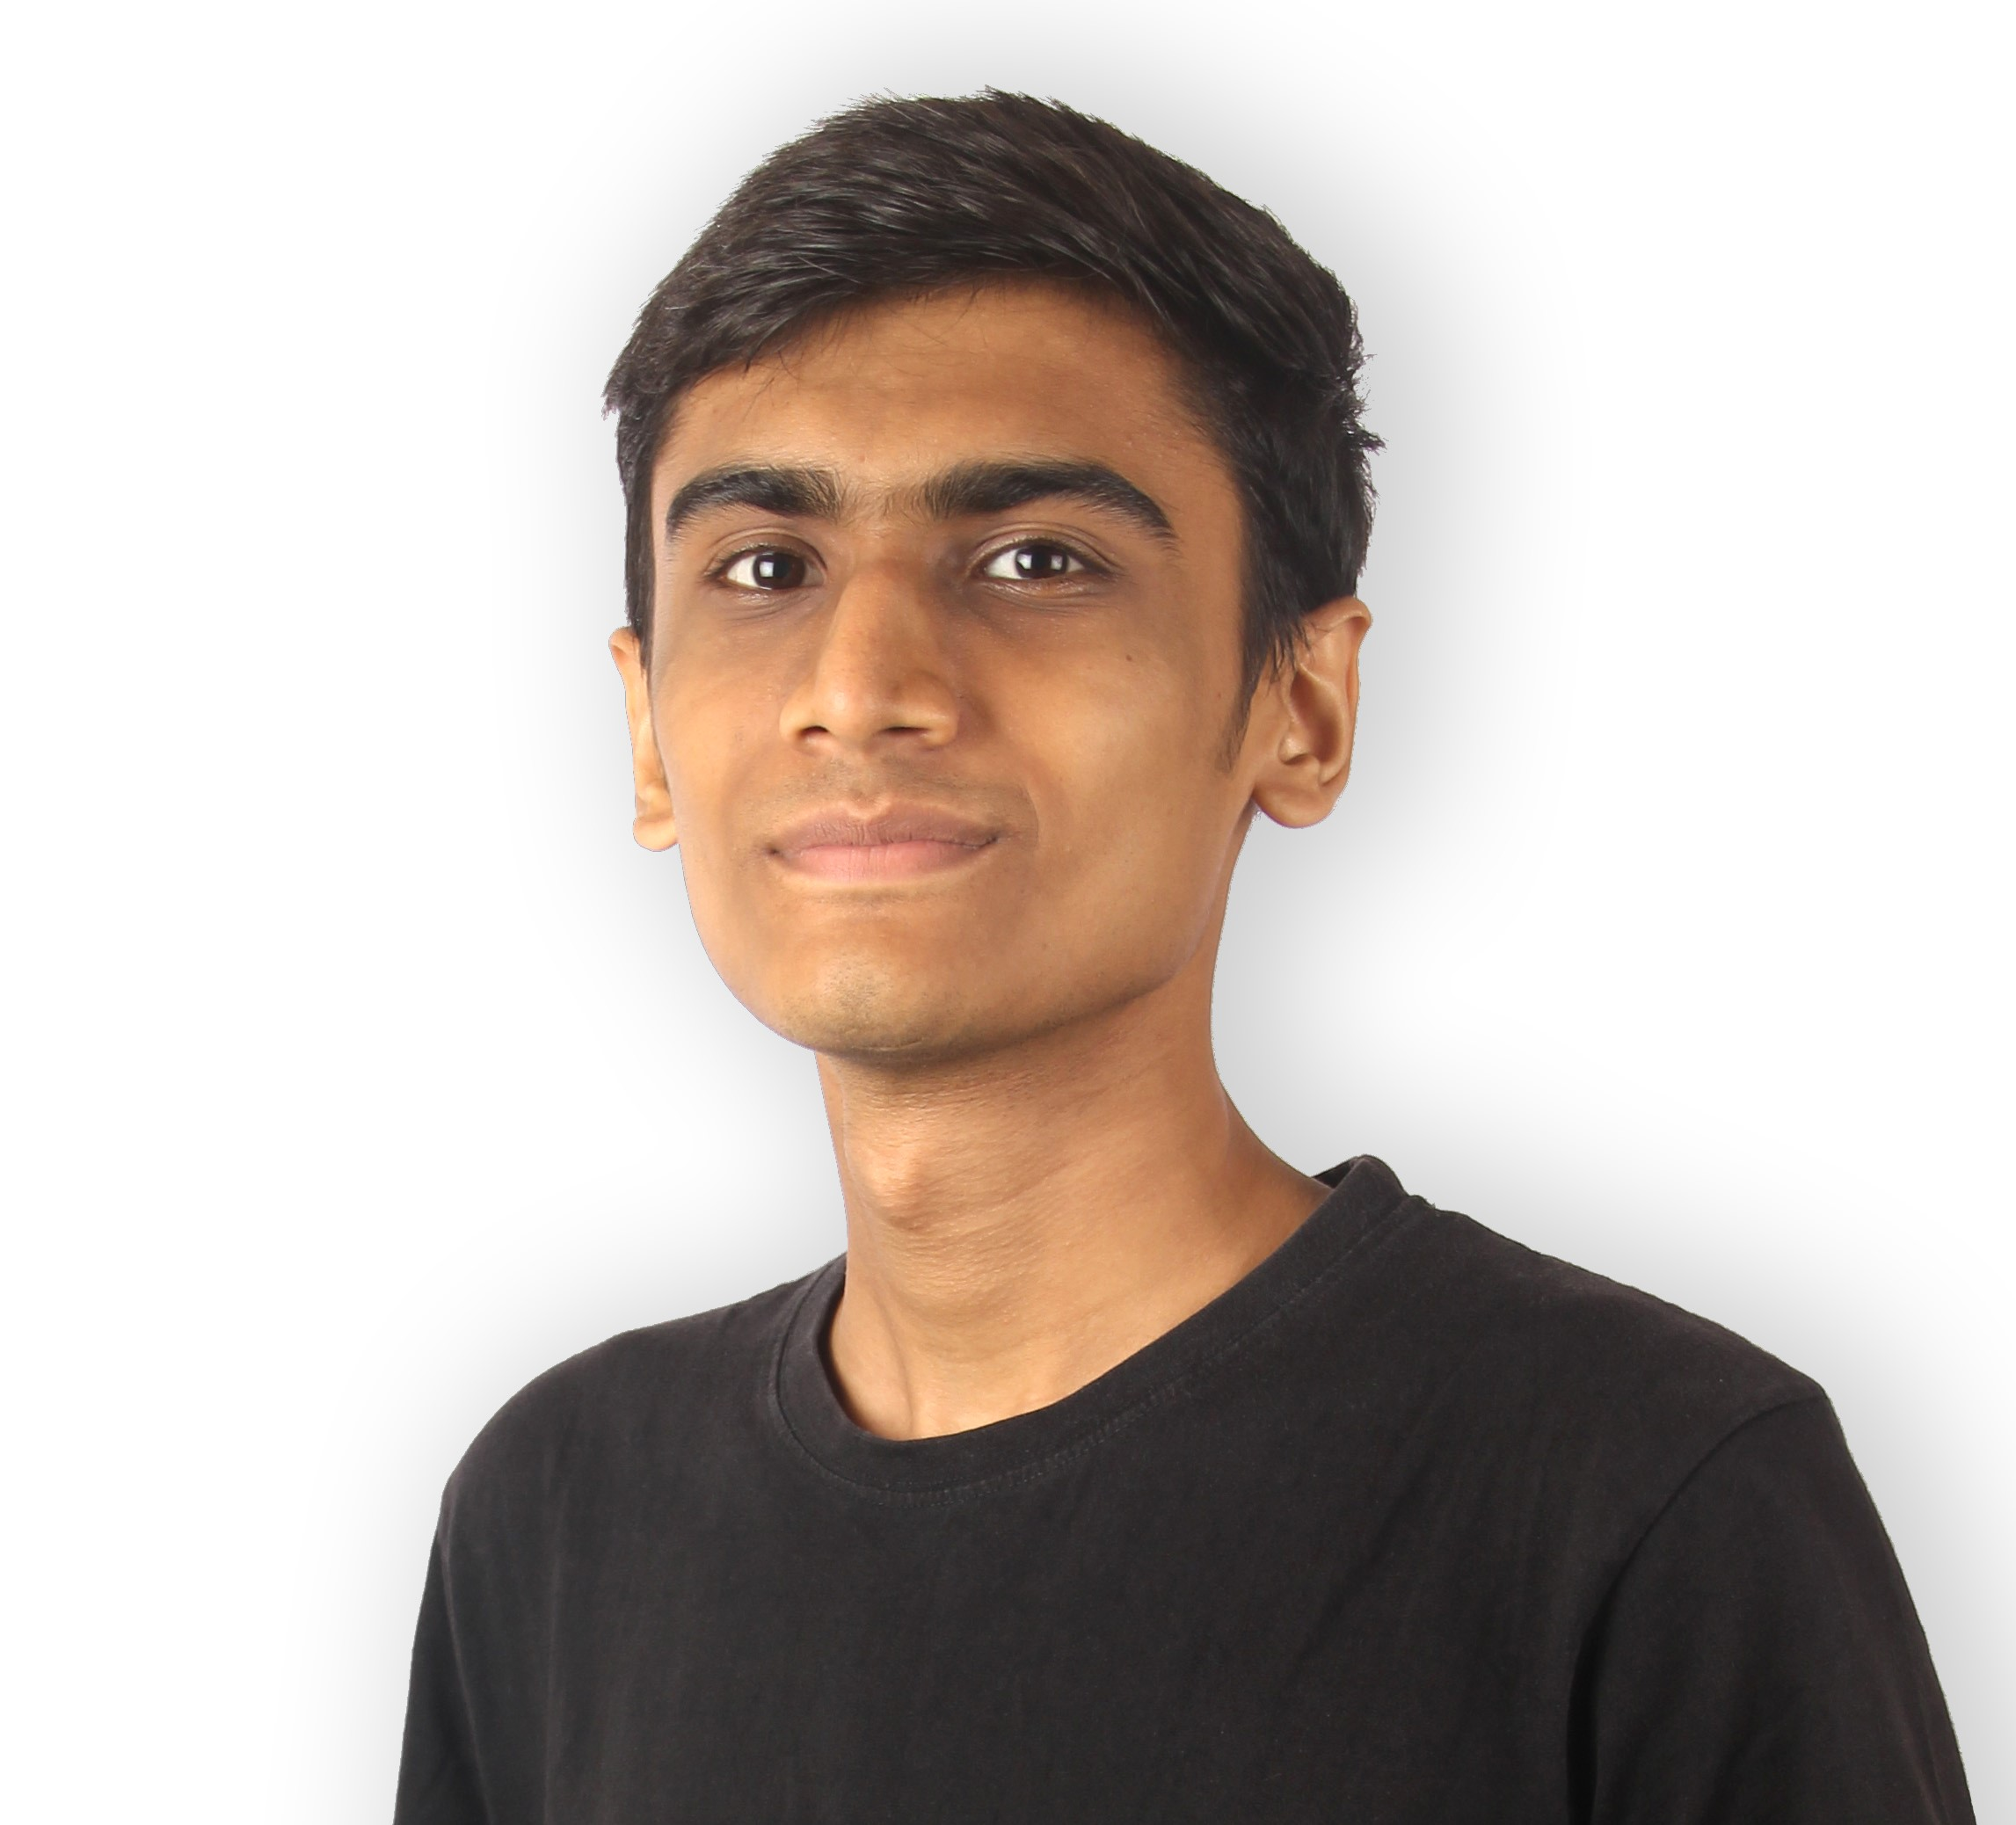
\includegraphics[height=2.5cm]{fig/lec01/Tatsat.jpg}
				\caption*{Tatsat Baldaniya}
		\end{figure}
		\column[T]{0.33\textwidth}
		\begin{figure}
			\centering
				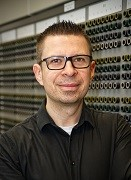
\includegraphics[height=2.5cm]{fig/lec01/pawel.jpg}
				\caption*{Pawel Malicki}
		\end{figure}		
	\end{columns}
	\vspace{-0.5cm}
	\begin{varblock}{Contact}
		\begin{itemize}
			\item Email: see chair's homepage \href{https://www.uni-siegen.de/ias}{www.uni-siegen.de/ias}
			\item Offices: H-A building, 4th floor
			\item Individual appointments on request (remote or personally)
            \item Multiple relevant courses are offered by the Chair.  \href{https://www.uni-siegen.de/ias-lehre-fak-iv/eti/vernetzte-automatisierungssysteme}{Check link!}
		\end{itemize}
	\end{varblock}
	\end{frame}


\begin{frame}{Necessary Prior Knowledge for this Course}
  \textbf{Students are expected to have a basic understanding of:}
  \begin{itemize}
    \item \textbf{Basic physics and laws governing systems:} for example, Newton's law of motion, electricity, dimensional consistency, etc.
    \item \textbf{Mathematical background:} algebra, complex numbers (phasors), basic calculus and elementary differential equations.
    \item \textbf{Basic signal theory:} Fourier series, Laplace transform, transfer functions, step/impulse response.
    \item \textbf{General systems thinking:} reading block diagrams, input-output viewpoints, feedback/feedforward concepts.
    \item \emph{No advanced programming is required -- any code used will be introduced as needed and tied to real automation tasks.}
  \end{itemize}

  \textbf{Topics not covered (addressed in other courses):}
  \begin{itemize}
    \item Machine learning in automation.
    \item Advanced control theory (e.g., optimal, robust, nonlinear control), robotics, etc.
  \end{itemize}
\end{frame}


\begin{frame}
	\frametitle{Recommended reading}
	\begin{itemize}
		\item Weyrich, Michael. Industrial Automation and Information Technology. Berlin, Germany: Springer, 2024.
		\item Daniel E.. Kandray. Programmable Automation Technologies: An Introduction to CNC, Robotics and PLCs. Industrial Press, 2010.
		\item Hering, Ekbert, and Gert Schönfelder. Sensors in Science and Technology. Springer Fachmedien Wiesbaden, 2022.
		\item Woods, Roger, John McAllister, Gaye Lightbody, and Ying Yi. FPGA-based implementation of signal processing systems. John Wiley \& Sons, 2008.
		\item Bartelt, Terry LM. Industrial automated systems: instrumentation and motion control. Delmar Learning, 2010.
	\end{itemize}
\end{frame}